\section{Описание использованного алгоритма}

\subsection{Описание алгоритма главного меню}
Для читаемости алгоритма логика отображения пунктов меню опущена,
а также убрана логика обработки статусов выполнения функций обработки массива.
Функции меню в блок-схеме алгоритма объединены в \texttt{initMenuDialog()}.

\begin{figure}[H]
  \centering
  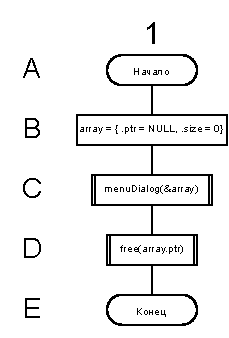
\includegraphics[width=0.35\textwidth]{fun_main}
  \caption{
    Блок-схема алгоритма работы функции 
    \texttt{main()}.
  }
\end{figure}

\begin{figure}[H]
  \centering
  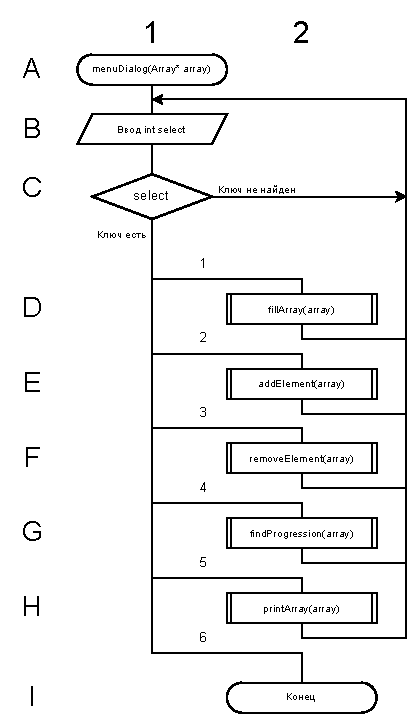
\includegraphics[width=0.45\textwidth]{fun_menu}
  \caption{
    Блок-схема алгоритма работы функций 
    \texttt{initMenuDialog()},
    \texttt{printMenuOptions()}, 
    \texttt{parseUserInput()} 
    и \texttt{exitMenuDialog()}.
  }
\end{figure}

\subsection{Описание алгоритма обратоки массивов}

% 1. Initialize new array 
\subsubsection{Описание алгоритма заполнения массива}

\begin{figure}[H]
  \centering
  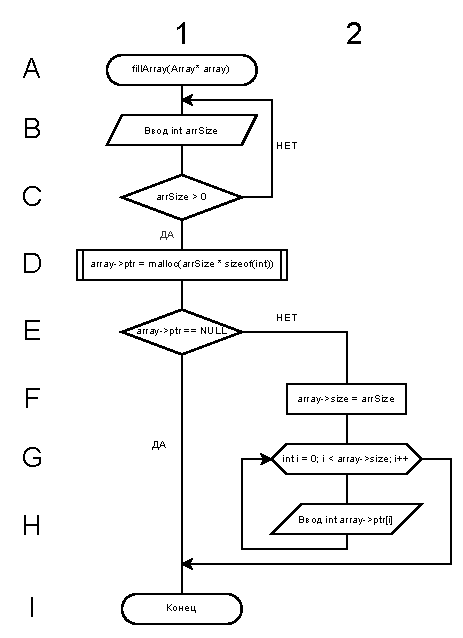
\includegraphics[width=0.35\textwidth]{fun_fillArray}
  \caption{
    Блок-схема алгоритма работы функции 
    \texttt{fillArray()}.
  }
\end{figure}

% 2. Append value to array by index
\subsubsection{Описание алгоритма добавление элемента в массив}

Алгоритм добавление элементов в массив разбит на две функции
из-за необходимости добавления элемента по определённому
индексу для функции \texttt{findProgression()}.

\begin{figure}[H]
  \centering
  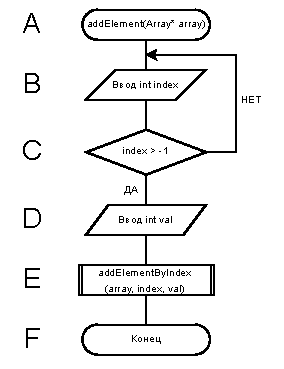
\includegraphics[width=0.35\textwidth]{fun_addElement}
  \caption{
    Блок-схема алгоритма работы функции.
    \texttt{addElement()}.
  }
\end{figure}

\begin{figure}[H]
  \centering
  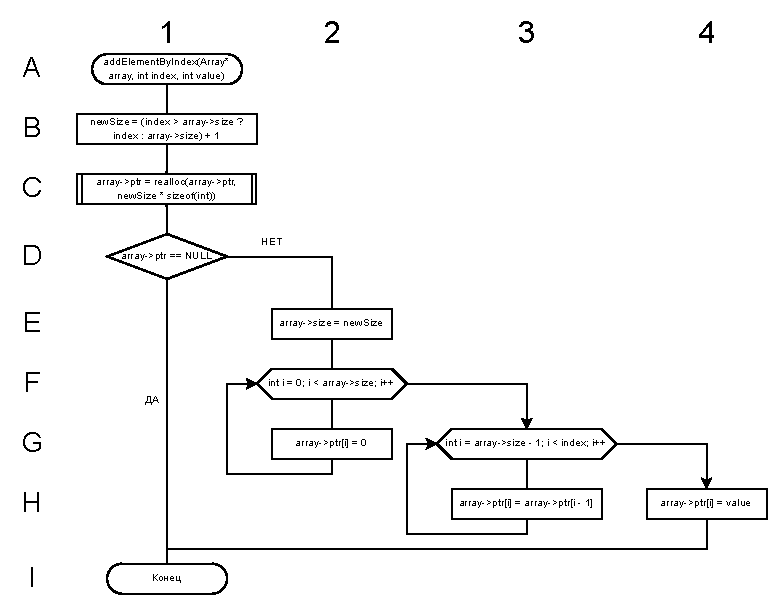
\includegraphics[width=0.8\textwidth]{fun_addElementByIndex}
  \caption{
    Блок-схема алгоритма работы функции.
    \texttt{addElementByIndex()}.
  }
\end{figure}

% 3. Delete value in array by index
\subsubsection{Описание алгоритма удаление элемента из массива}

Алгоритм добавление элементов в массив разбит на две функции
по аналогичных причинам для функции \texttt{findProgression()}.

\begin{figure}[H]
  \centering
  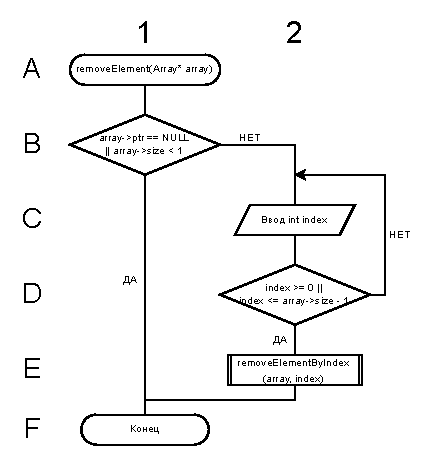
\includegraphics[width=0.4\textwidth]{fun_removeElement}
  \caption{
    Блок-схема алгоритма работы функции.
    \texttt{removeElement()}.
  }
\end{figure}

\begin{figure}[H]
  \centering
  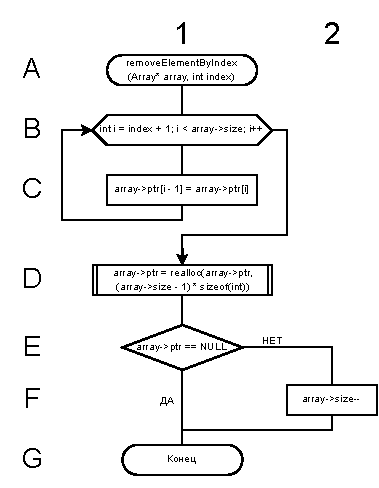
\includegraphics[width=0.35\textwidth]{fun_removeElementByIndex}
  \caption{
    Блок-схема алгоритма работы функции.
    \texttt{removeElementByIndex()}.
  }
\end{figure}

% 4. Find arithmetic progression
\subsubsection{Описание алгоритма поиска арифметической прогрессии в цифрах элементов массива}

\begin{figure}[H]
  \centering
  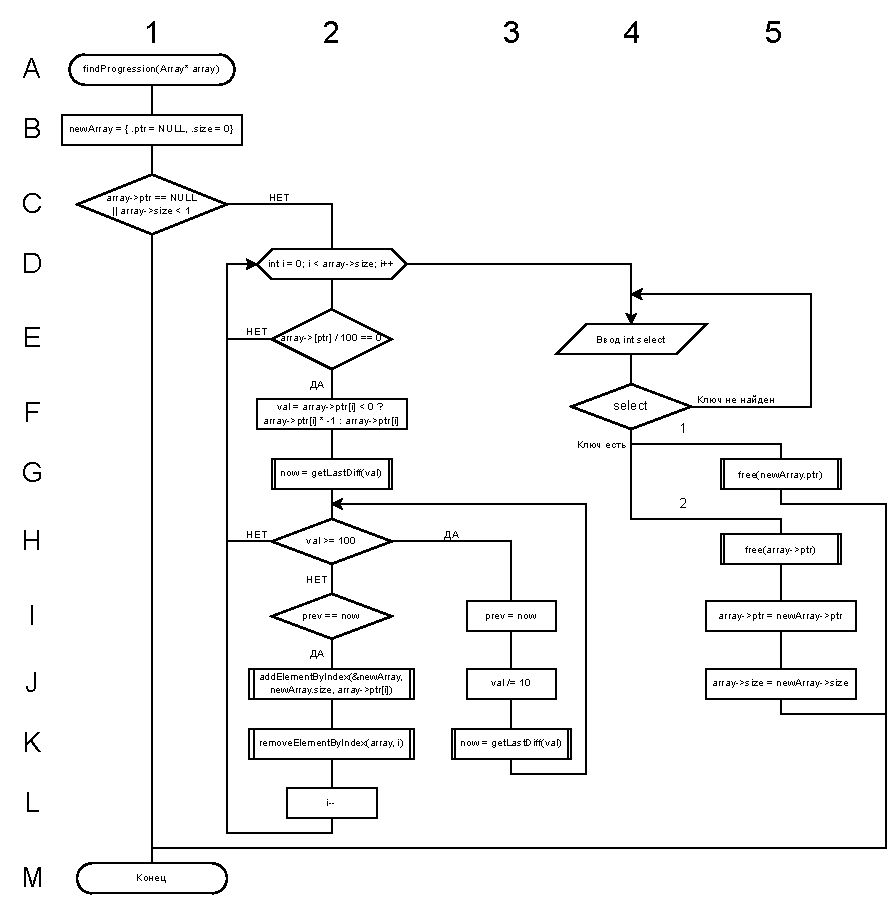
\includegraphics[width=0.75\textwidth]{fun_findProgression}
  \caption{
    Блок-схема алгоритма работы функции.
    \texttt{findProgression()}.
  }
\end{figure}

\begin{figure}[H]
  \centering
  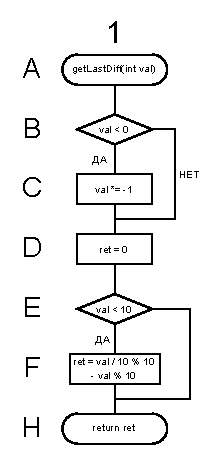
\includegraphics[width=0.3\textwidth]{fun_getLastDiff}
  \caption{
    Блок-схема алгоритма работы функции.
    \texttt{getLastDiff()}.
  }
\end{figure}

% 5. Print current array
\subsubsection{Описание алгоритма вывода массива}

По сравнению с реализованной функцией в блок-схеме алгоритма
отсутствует вывод размера массива и дополнительных символов для удобства.

\begin{figure}[H]
  \centering
  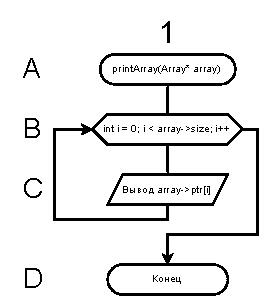
\includegraphics[width=0.35\textwidth]{fun_printArray}
  \caption{
    Блок-схема алгоритма работы функции.
    \texttt{printArray()}.
  }
\end{figure}
